\icode{E-MD-MU-L3-261120-003}
（多选）
如图是一种升降系统示意图。轻弹簧上端固定质量为 \(m\) 的平台，站在上面的人手握轻质横杆，绳子的一端与横杆相连，另一端与定滑轮相连，初始时绳子刚好伸直但无张力，人和平台处于静止状态。启动电动机，让其带动定滑轮向上收绳子，使人和平台一起做加速度为 \(a\) 的匀加速直线运动，直至人离开平台。已知弹簧劲度系数为 \(k\)，人的质量为 \(M\)，重力加速度为 \(g\)。下列说法正确的是\paren[]

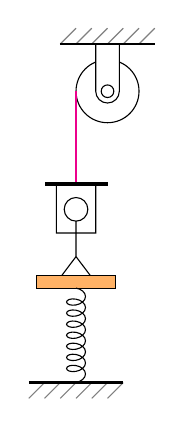
\begin{tikzpicture}
	\fill (-.4,0) rectangle(.4,.05);
	\draw (0,-.3) circle(.15);
	\draw (0,-.45)--(0,-.9)--++(-127:.3) (0,-.9)--++(-53:.3) (-.25,0)--(-.25,-.6)--(.25,-.6)--(.25,0);
	\draw (.4,1.2) circle(.4); 
	\draw[fill=white](.25,1.8)--(.25,1.2) arc(-180:0:.15)--(.55,1.8);
	\draw (.4,1.2) circle(.08);
	\draw[magenta] (0,.05)--(0,1.2);
	\draw[fill=orange!60] (-.5,-1.14) rectangle(.5,-1.3);
	\draw[decoration={aspect=.6,segment length=4,amplitude=1.2mm,coil},decorate] (0,-1.3)--(0,-2.5);
	\foreach \x in {-.2,0,...,.8}
		\draw[gray] (\x,1.8)--++(.2,.2);
	\foreach \x in {-.6,-.4,...,.6}
		\draw[gray] (\x,-2.7)--++(.2,.2);
	\draw[thick] (-.6,-2.5)--(.6,-2.5) (-.2,1.8)--(1,1.8);
\end{tikzpicture}
\begin{choices}
	\item 电动机启动前，弹簧的形变量为 \(\dfrac{(M+m)g}{k}\)
	\item 电动机启动瞬间，绳子拉力大小为 \((M+m)g\)
	\item 人与平台分离瞬间，弹簧的形变量为 \(\dfrac{M(g+a)}{k}\)
	\item 当平台速度达到最大时，平台上升的高度为 \(\dfrac{Mg}{k}\)
\end{choices}
\begin{answer}
	AD\qquad 提示：
\end{answer}